\documentclass[12pt, a4paper]{article}
\usepackage[T2A]{fontenc}
\usepackage[utf8]{inputenc}
\usepackage[russian]{babel}
\usepackage{graphicx}
\usepackage{geometry}
\usepackage{textpos}
\usepackage{textpos}
\usepackage{array}
\usepackage{caption}
\usepackage{amsmath}
\usepackage{fancyhdr}
\usepackage{listings}
\usepackage{xcolor}

% Дефайним цвета под листинги
\definecolor{codegreen}{rgb}{0,0.6,0}
\definecolor{codegray}{rgb}{0.5,0.5,0.5}
\definecolor{codepurple}{rgb}{0.58,0,0.82}
\definecolor{backcolour}{rgb}{0.95,0.95,0.92}

% Задаем стиль под сам листинг
\lstdefinestyle{mystyle}{
	backgroundcolor=\color{backcolour},   
	commentstyle=\color{codegreen},
	keywordstyle=\color{magenta},
	numberstyle=\tiny\color{codegray},
	stringstyle=\color{codepurple},
	basicstyle=\ttfamily\footnotesize,
	breakatwhitespace=false,         
	breaklines=true,                 
	captionpos=b,                    
	keepspaces=true,                 
	numbers=left,                    
	numbersep=5pt,                  
	showspaces=false,                
	showstringspaces=false,
	showtabs=false,                  
	tabsize=2
}

\lstset{style=mystyle}

\geometry{
	a4paper,
	textwidth=170mm,
	textheight=250mm,
	left=20mm,
	top=20mm,
}

\newcommand{\Faculty}{Робототехника и комплексная автоматизация}
\newcommand{\Department}{Системы автоматизированного проектирования (САПР)}

\newcommand{\TitleText}{Отчет о выполнении домашней работы}
\newcommand{\Title}{{\Huge \textbf{\TitleText}}}

\newcommand{\SubTitleText}{по дисциплине "Модели и методы анализа проектных решений"}
\newcommand{\SubTitle}{{\LARGE \textbf{\SubTitleText}}}

\newcommand{\FullName}{Дунайцев Александр Иванович}
\newcommand{\Author}{Дунайцев А. И}
\newcommand{\EduGroup}{РК6-64Б}
\newcommand{\TaskType}{Вариант 67}
\newcommand{\WorkTheme}{Метод конечных разностей при решении задач теплопроводности}

% Пример как добавить картину в документ
%\begin{figure}[h]
%	\centering    % Центрируем
%	\includegraphics[width=0.25\textwidth]{pic.png}
%	\caption{a nice plot} % Подписть к картинке, будет снизу
%	\label{fig:pic1} % Можно указывать ссылку на эту картинку в тексте, как \ref{fig:pic1}
%\end{figure}

% Так можно вставить листинг ин плейс
%\begin{lstlisting}[language=Python]
%	...
%\end{lstlisting}

% Так можно вставить листинг 
%\lstinputlisting[language=C]{BitXorMatrix.c}



\setlength{\columnsep}{1in}


\begin{document}
	% Место для верстки титульного документа
	\thispagestyle{empty}
	\begin{tabular}{m{0.15\linewidth}m{0.85\linewidth}}
	\centering
	
\includegraphics[scale=0.07]{static/bmstu.pdf} &
	{\centering
	Министерство науки и высшего образования Российской Федерации
	Федеральное государственное бюджетное образовательное учреждение
	высшего образования
	
	«Московский государственный технический университет
	имени Н.Э. Баумана
	(национальный исследовательский университет)»
	
	(МГТУ им. Н.Э. Баумана)
	
    } \\
	\hline
	\multicolumn{1}{p{0.15\textwidth}}{} & \multicolumn{1}{p{0.85\textwidth}}{} \\
	\multicolumn{1}{p{0.15\textwidth}}{ФАКУЛЬТЕТ}	&	\multicolumn{1}{p{0.85\textwidth}}{\Faculty}	\\
	\multicolumn{1}{p{0.15\textwidth}}{КАФЕДРА}	&	\multicolumn{1}{p{0.85\textwidth}}{\Department}	\\
	\end{tabular}
\vfil

\begin{center}
	\Title
	
	\SubTitle
\end{center}


\vfil
\begin{center}
	\begin{tabular}{p{0.4\textwidth}p{0.4\textwidth}} 
		Студент:	& \FullName \\ 
		\hline
		Группа:	& \EduGroup \\ 
		\hline
		Тип задания:	& \TaskType \\ 
		\hline
		Тема:	& \WorkTheme \\ 
		\hline
	\end{tabular}
\end{center}

\vfil

\begin{tabular}{p{0.45\textwidth}p{0.25\textwidth}p{0.25\textwidth}} 
	\large
	Студент	&	$\underset{\text{подпись, дата}}{\underline{\hspace{0.2\textwidth}}}$ & \underline{\Author}  \\ 
	& & \\
	Преподаватель	&	$\underset{\text{подпись, дата}}{\underline{\hspace{0.2\textwidth}}}$ & \underline{Трудоношин В. А.} \\ 
\end{tabular}

\vfil
\vfil
\begin{center}
	Москва, 2022
\end{center}

%Конец титульного листа
\newpage	
	% Страница с версткой содержания
	\tableofcontents
	\newpage
	
	% Далее идут секции с текстом документа
	\section{Задание}
	С помощью явной разностной схемы решить нестационарное уравнение теплопроводности для трубы, изображенной на рис. \ref{fig:pic1}, там же указаны размеры сторон.
	
	\begin{figure}[h]
		\centering    % Центрируем
		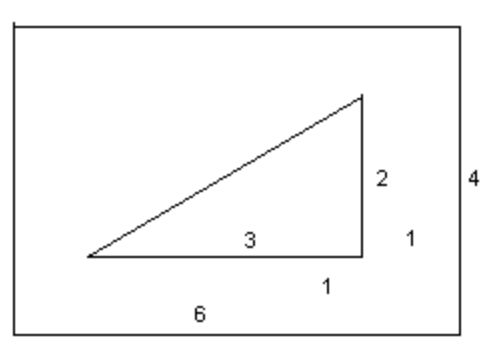
\includegraphics[width=0.6\textwidth]{static/task.png}
		\caption{Форма трубы} % Подписть к картинке, будет снизу
		\label{fig:pic1} % Можно указывать ссылку на эту картинку в тексте, как \ref{fig:pic1}
	\end{figure}

    Граничные условия:
    Внутри трубы задано условие: $\frac{\partial T}{\partial n} = T$.
    
    На внешних границах заданы следующие условия: верхняя сторона - 20, на остальных выполняется условие $\frac{\partial T}{\partial n} = 40$.
    
    Начальное значение температуры трубы - 20 градусов.
    
    При выводе результатов показать динамику изменения температуры (например, с помощью цветовой гаммы).
	
	\section{Теоретическая часть}
	\subsection{Нестационарное уравнение теплопроводности}
	
	В отличие от стационарных задач, при постановке нестационарных задач нас интересует определение состояния сплошной среды переменное во времени. Для решения подобного рода задач определяют краевые условия, то есть совокупность граничных условий и условий состояния среды в начальный момент времени (начальных условий).
	
	В контексте поставленной задачи необходимо найти значения температуры всех точек среды (в данном случае трубы), в разные моменты времени. Совокупность значений температуры во всех точках среды в определенный момент времени называют температурным полем.
	
	Для решения двумерных задач, связанных с поиском значений температурного поля в различные моменты времени, необходимо иметь дифференциальное уравнение теплопроводности пластины, которое связывает температуру пластины, время и пространственными координатами исследуемой среды. В декартовой системе координат такое урпанение имеет следующий вид:
	
	\[
	\frac{\partial T}{\partial t} = \frac{\lambda}{cp}\left( \frac{\partial^2 T}{\partial x^2}  + \frac{\partial^2 T}{\partial y^2} \right) + \frac{w}{cp},
	\]
	
	где $\lambda$ - коэфициент теплопроводности, $c$ - теплоемкость, $p$ - плотность, $w$ - мощность тепловыделения.
	
	\subsection{Метод конечных разностей}
	Для решения поставленной задачи воспользуемся методом конечных разностей (далее МКР).
	
	Смысл этого метода заключается в представлении исходного объекта его математическим аналагом, который представляет сосбой сетку, в узлах которой находятся исследуемые значения. Каждый узел соответствует значению в определенной простарнственной координате исходного объекта, таким образом координата узла вычисляется следующим $(x_i, y_j) = (i\Delta x, j\Delta y)$, где $i \in [0, ..., n]$, $j \in [0, ... m]$, а $n, m$ - количество узлов вдоль оси абсцисс и оси ординат соответственно.
	
	Далее можно перейти к разностным аналогам частных проивзодных в двумерном пространстве. Записать их можно следующим образом:
	Первая производная
	
	\[
	\frac{\partial T}{\partial y} = \frac{T^k_{i, j + 1} - T^k_{i,j}}{\Delta y}
	\]
	
	Вторая производная
	
	\[
	\frac{\partial^2 T}{\partial y^2} = \frac{T^k_{i, j + 1} - 2T^k_{i,j} + T^k_{i,j-1}}{\Delta y^2}.
	\]
	
	Здесь $k$ - это индекс узла по времени, $i$ - индекс узла по координате $x$, $j$ - индекс по координате $y$.
	Важно отметить, что в данном примере записи разностной формы производная берется по координате $y$. Однако в зависимости от переменной, по которой берется производная, будет изменяться индекс в разностной схеме, соответствуюший этой переменной.
	
	Таким образом, можно записать уравнение теплопроводности с помощью явной разностной схемы следующим образом:
	
	\[
	\frac{T^{k + 1}_{i, j} - T^k_{i,j}}{\Delta t} = \frac{\lambda}{cp} \left( \frac{T^k_{i + 1, j} - 2T^k_{i,j} + T^k_{i - 1,j}}{\Delta x^2} + \frac{T^k_{i, j + 1} - 2T^k_{i,j} + T^k_{i,j-1}}{\Delta y^2} \right) + \frac{w}{cp}.
	\]
	
	Так как исследуемый объект имеет отверстие в центре неправильной формы, имеет смысл брать сетку таким образом, чтобы ее узлы оказывались на границах треугольного отверстия в центре трубый.
	
	Уравнения граничных условий также записываются в виде своих разностных аналогов.
	
	ГУ 1-го рода для верхней грани трубы:
	\[
	T = 20
	\]
	
	ГУ 2-го рода для правой ли левой грани трубы:
	\[
	\frac{T_{i-1,j} - T_{i,j}}{\Delta x} = 40,
	\]
	\[
	\frac{T_{i+1,j} - T_{i,j}}{\Delta x} = 40
	\]
	
	ГУ 2-го рода для нижней грани трубы:
	\[
	\frac{T_{i,j-1} - T_{i,j}}{\Delta y} = 40
	\]
	
	Внтури трубы задано ГУ 3-го рода.
	На границах отверстия, параллельных осям системы коодринат:
	\[
	\frac{T_{i,j-1} - T_{i,j}}{\Delta y} = T_{i,j}
	\]
	\[
	\frac{T_{i+1,j} - T_{i,j}}{\Delta x} = T_{i,j}
	\]
	
	Для записи ГУ на наклонной грани отверстия введем переменную $h = \sqrt{\Delta x^2 + \Delta y^2}$. Тогда ГУ 3-го рода на этой грани можно записать так:
	\[
	\frac{T_{i+1,j+1} - T_{i,j}}{h} = T_{i,j}
	\]
	
	\section{Описание работы программы}
	
	Решение нестационарного уравнения теплопроводности сводится к тому, чтобы на всех временных слоях получить получить значения во всех узлах сетки заданой модели.
	
	Чтобы задать сетку, довольно удобно воспользоваться двумерным массивом, который учитывает форму исследуемого объекта. Таким образом, каждая ячейка массива будет хранить в себе значение узла. Однако, поскольку хранение двумерного массивабольшого в памяти компьютера довольно накладно по скорости доступа к элементу массива, следует заменить двумерный массив на одномерный, класс которого будет иметь семантику работы двумерного массива.
	
	После создания сетки, решение поставленной задачи сводится к итерационному вычислению значений всех узлов сетки на всех временных слоях. Следует отметить, что при этом учитываются граничные условия заданные на исследуемый объект.
	
	Решение нестационарных задач теплопроводности может оказаться достаточно затратным по памяти, при условии, что заданы достаточно маленькие приращения по пространственным координатам и большое количество временных слоев. В связи с этим программная реализация должна сводится только к рассчетам на всех временных слоях, а не попыткам сохранить их в оперативной памяти компьютера, поэтому реализованый класс модели не отвечает за хранение вычислений. Он лишь принимает полиморфный объект хранилища, который отвечает за сохранение результата рассчетов, если это необходимо.
	
	\section{Решение задачи}
	\subsection{Решение задачи с помощью разработанной программы}
	
	Для более наглядного отображения работы программы, было принято решение задать температуру внутри трубы равной 0 градусам. Однако, следует отметить, что значения внутри трубы никак не учитываются и не виляют на граничные условия, заданные на границах отверстия. В результате интегрирования по времени в течении 25 секунд, получилась тепловая карта, представленная на рисунке \ref{fig:pic2}. 
	
	\begin{figure}[h]
		\centering    % Центрируем
		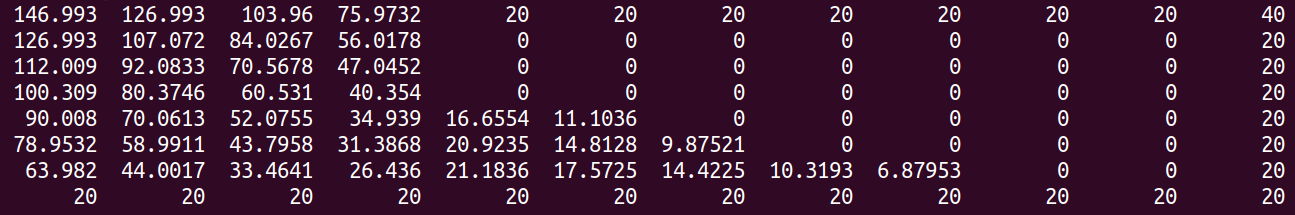
\includegraphics[width=0.6\textwidth]{static/TableResult.png}
		\caption{Результат работы программы в табличном виде с шагом h = 0.5} % Подписть к картинке, будет снизу
		\label{fig:pic3} % Можно указывать ссылку на эту картинку в тексте, как \ref{fig:pic1}
	\end{figure}
	
	\begin{figure}[h]
		\centering    % Центрируем
		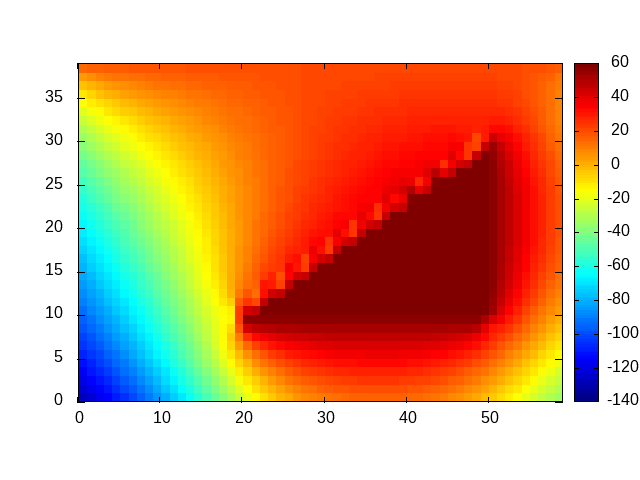
\includegraphics[width=0.6\textwidth]{static/heatmap.png}
		\caption{Графическое изображение результатов рассчетов с шагом 0.1} % Подписть к картинке, будет снизу
		\label{fig:pic2} % Можно указывать ссылку на эту картинку в тексте, как \ref{fig:pic1}
	\end{figure}

    \subsection{Решение задачи с помощью пакета ANSYS}
    Для решения задачи теплопроводности трубы средствами покета ANSYS, была построена модель трубы, проведено разбиение на конечные элементы, наложены граничные условия. Визуализация распределения температур для момента времени t = 25 сек представлена на рисунке \ref{fig:pic4}.
    
    \begin{figure}[h]
    	\centering    % Центрируем
    	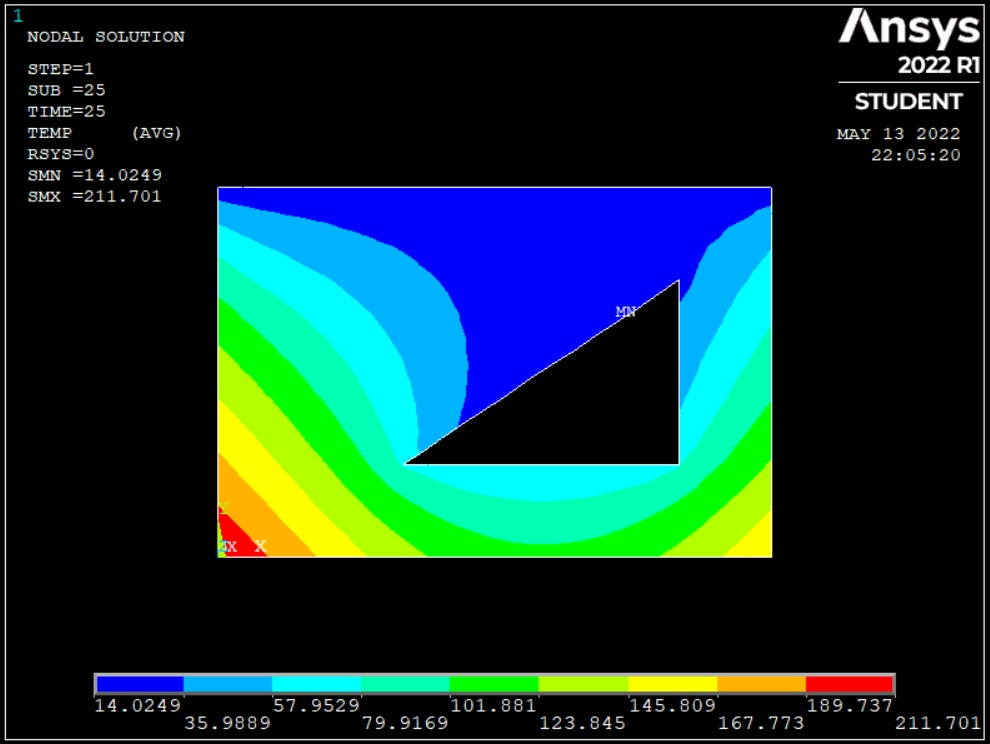
\includegraphics[width=0.6\textwidth]{static/AnsysResult.jpg}
    	\caption{Графическое изображение результатов рассчетов с помощью ANSYS} % Подписть к картинке, будет снизу
    	\label{fig:pic4} % Можно указывать ссылку на эту картинку в тексте, как \ref{fig:pic1}
    \end{figure}

    \subsection{Сравнение резултатов работы программы}
    На основе полученных распределений температур, представленных на рисунке \ref{fig:pic4} и рисунке \ref{fig:pic3}, можно сделать вывод, что решение задачи при помощи пакета ANSYS и при помощи написанной программы совпадает. Отсюда можно заключить, что программа, реализованная в рамках данной работы, работает корректно.
	
	\section{Код программы}
	
	\subsection{Matrxix}
	\lstinputlisting[language=C++, caption={Matrix.hpp}]{../project/include/Matrix.hpp}
	
	\subsection{CalculationUtils}
	\lstinputlisting[language=C++, caption={CalculationUtils.hpp}]{../project/include/CalculationUtils.hpp}
	
	\subsection{SolutionStorage}
	\lstinputlisting[language=C++, caption={SolutionStorage.hpp}]{../project/include/SolutionStorage.hpp}
	
	\subsection{Model}
	\lstinputlisting[language=C++, caption={Model.hpp}]{../project/include/Model.hpp}
	\lstinputlisting[language=C++, caption={Model.cpp}]{../project/src/Model.cpp}
	
	\subsection{Решение задачи при помощи реализованных библиотек}
	\lstinputlisting[language=C++, caption={solution.cpp}]{../project/solution.cpp}
	
	
\end{document}